%************************************************
\chapter{Purification by Derivatisation and Crystallization}
%************************************************
\begin{flushright}
March 25, 2013
\end{flushright}
\section{Aim}
To separate Benzaldehyde by forming its Hydrazone derivative and then crystalling it out to recover its pure form.

\section {Chemicals Required}
	% \begin{figure}[bth]
	% 	\begin{center}
	% 		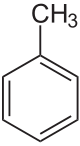
\includegraphics[width=0.1\linewidth]{gfx/e7_compound}
	% 	\end{center}
	% \caption[Aniline]{\label{e7_compound}}
	% \end{figure}


	\begin{enumerate}
		\item Benzaldehyde
		\item 2,4 - DNP
		\item Methanol
		\item Ethanol
		\item $H_2SO_4$ (catalyst)
	\end{enumerate}

\section{Theory}
	Derivitisation is a technique that's used in chemistry, for transforming a chemical compound into a derivative of itself, viz. a chemically similar product.
	\par
	Formation of 2,4-Dinintrophenylhydrazones from carbonyls, though more commonly from Aldehydes and 2,4 - DNP, is a very common method of derivatisation.
	\par
	The hydrazone forms orange crystals which may be purified by recrystallization.
	\par
	The reaction is carried out in an acidic medium.
	\par
	Recrystallisation is a technique often used to purify chemicals by dissolving them in an appropriate solvent, and as the name suggests, precipitating them to form crystals, while leaving out the impurities in the solution.

\section{Procedure}
	\begin{enumerate}
		\item A solution of benzaldehyde and methanol was taken in a beaker. And the solution of 2, 4-Dinintrophenylhydrazine, sulpuric acid and methanol in another.
		\item To the benzaldehyde solution, added was 2,4 - DNPH dropwise, while stirring was performed continueously.
		\par
			\emph{An orange precipitate was observed alongside.}
		\item Filtered the solution. From the solute thereby obtained, taken was a small amount, and dissolved it was in ethanol.
		\item Placed was this solution of hydrazone derivative, in ethanol on a water bath and heated it was, to approximately $80 ^O C$.
		\par
			\emph{A priorly observed orange precipitate now was found to have just dissolved, creating a saturated solution}			
		\item Filtered was the hot solution, with care.
		\item Kept was the filtrate to allow cooling, in an ice bath.
		\par
			\emph{An orange precipitate of hydrazone derivate of benzaldehyde was observed, however crystals were NOT observed}
	\end{enumerate}

\section{Observations and Results}
	The derivate of Benzaldehyde was created successfully, however its purification by recrystallization failed.

\section{Causes of failure}
	Perhaps the immediate cooling is what resulted in the failure of the recrystallization process. Another possibility is that the dissolution wasn't complete, which may have interfered the process of forming crystals.

\section{Precaution}
	\begin{enumerate}
		\item The heating was done indirectly again, since the substances are flammable
		\item Special care was taken, especially while handling methanol
	\end{enumerate}

	
\section{Acknowledgements}
I thank Dr. R Vijaya Anand for his guidance during the experiment. I also acknowledge the contribution of my lab partners, Srijit, Prashansa and Vivek for performance of the same. I also thank our PhD guide for demonstrating the experiment and her assistance in general, with performance of the same.

	% \clearpage
	% \begin{figure}[bth]
	% 	\begin{center}
	% 		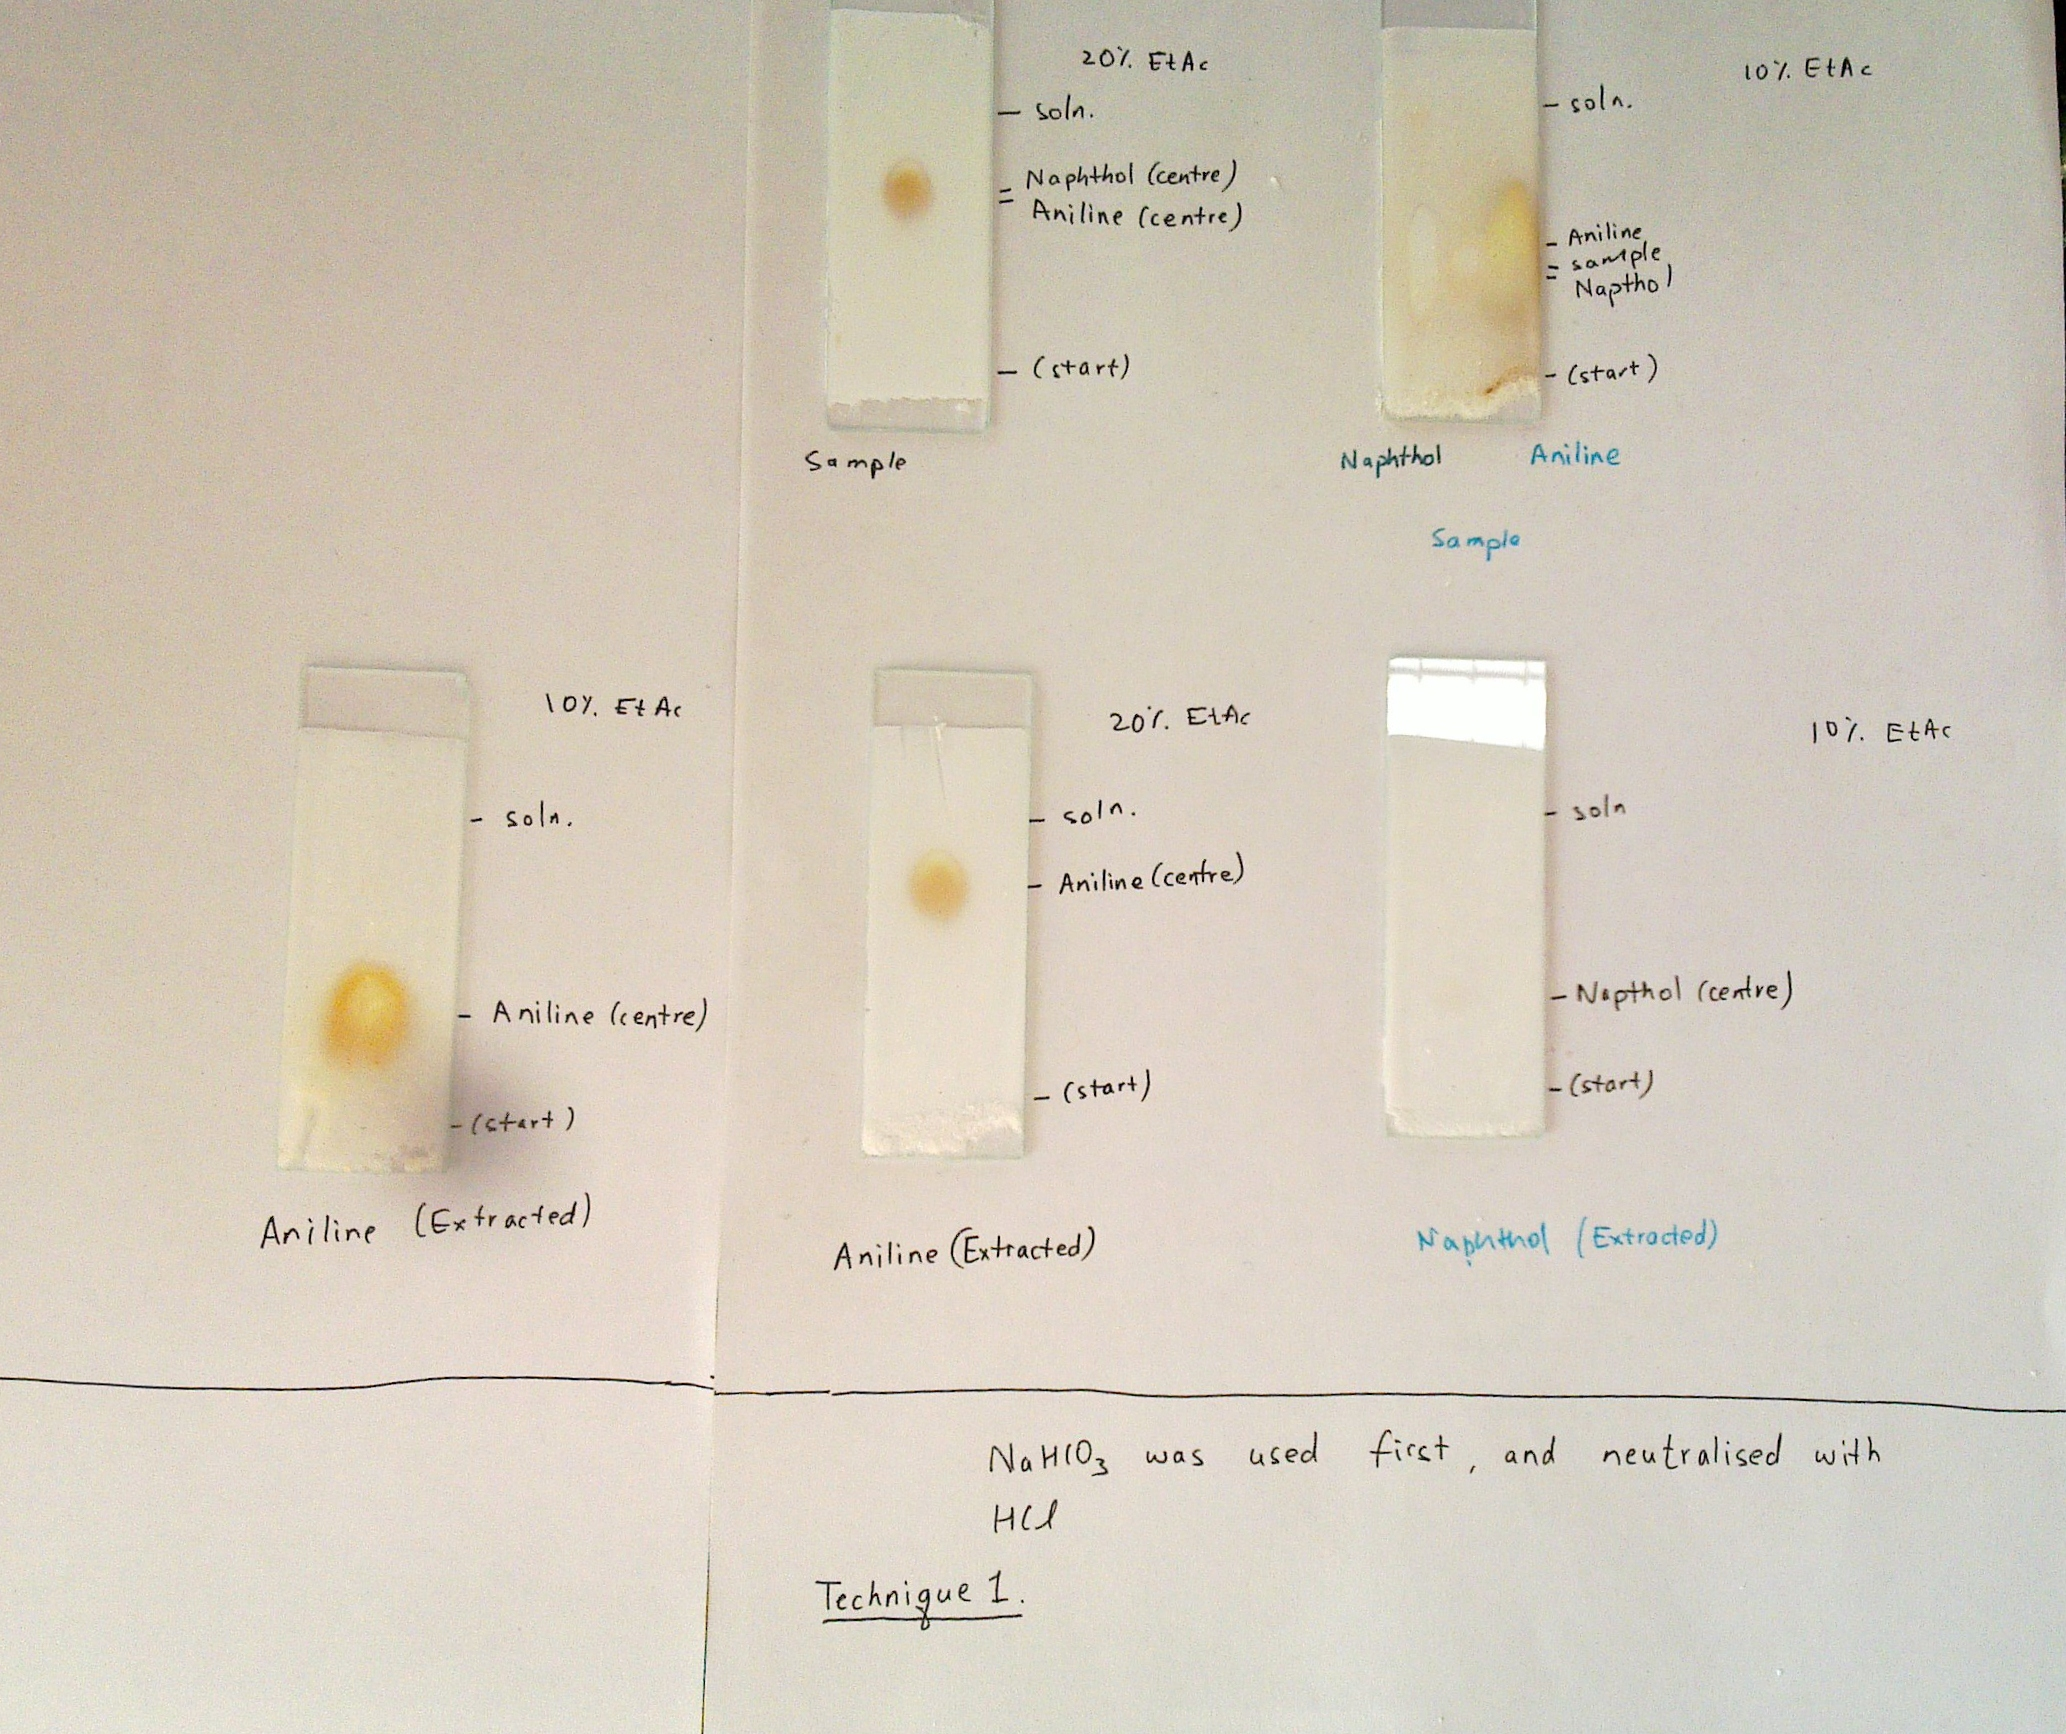
\includegraphics[width=1.5\linewidth]{gfx/e5_1}
	% 	\end{center}
	% \caption[TLCs Set 1]{\label{e5_1}}
	% \end{figure}

	% \begin{figure}[bth]
	% 	\begin{center}
	% 		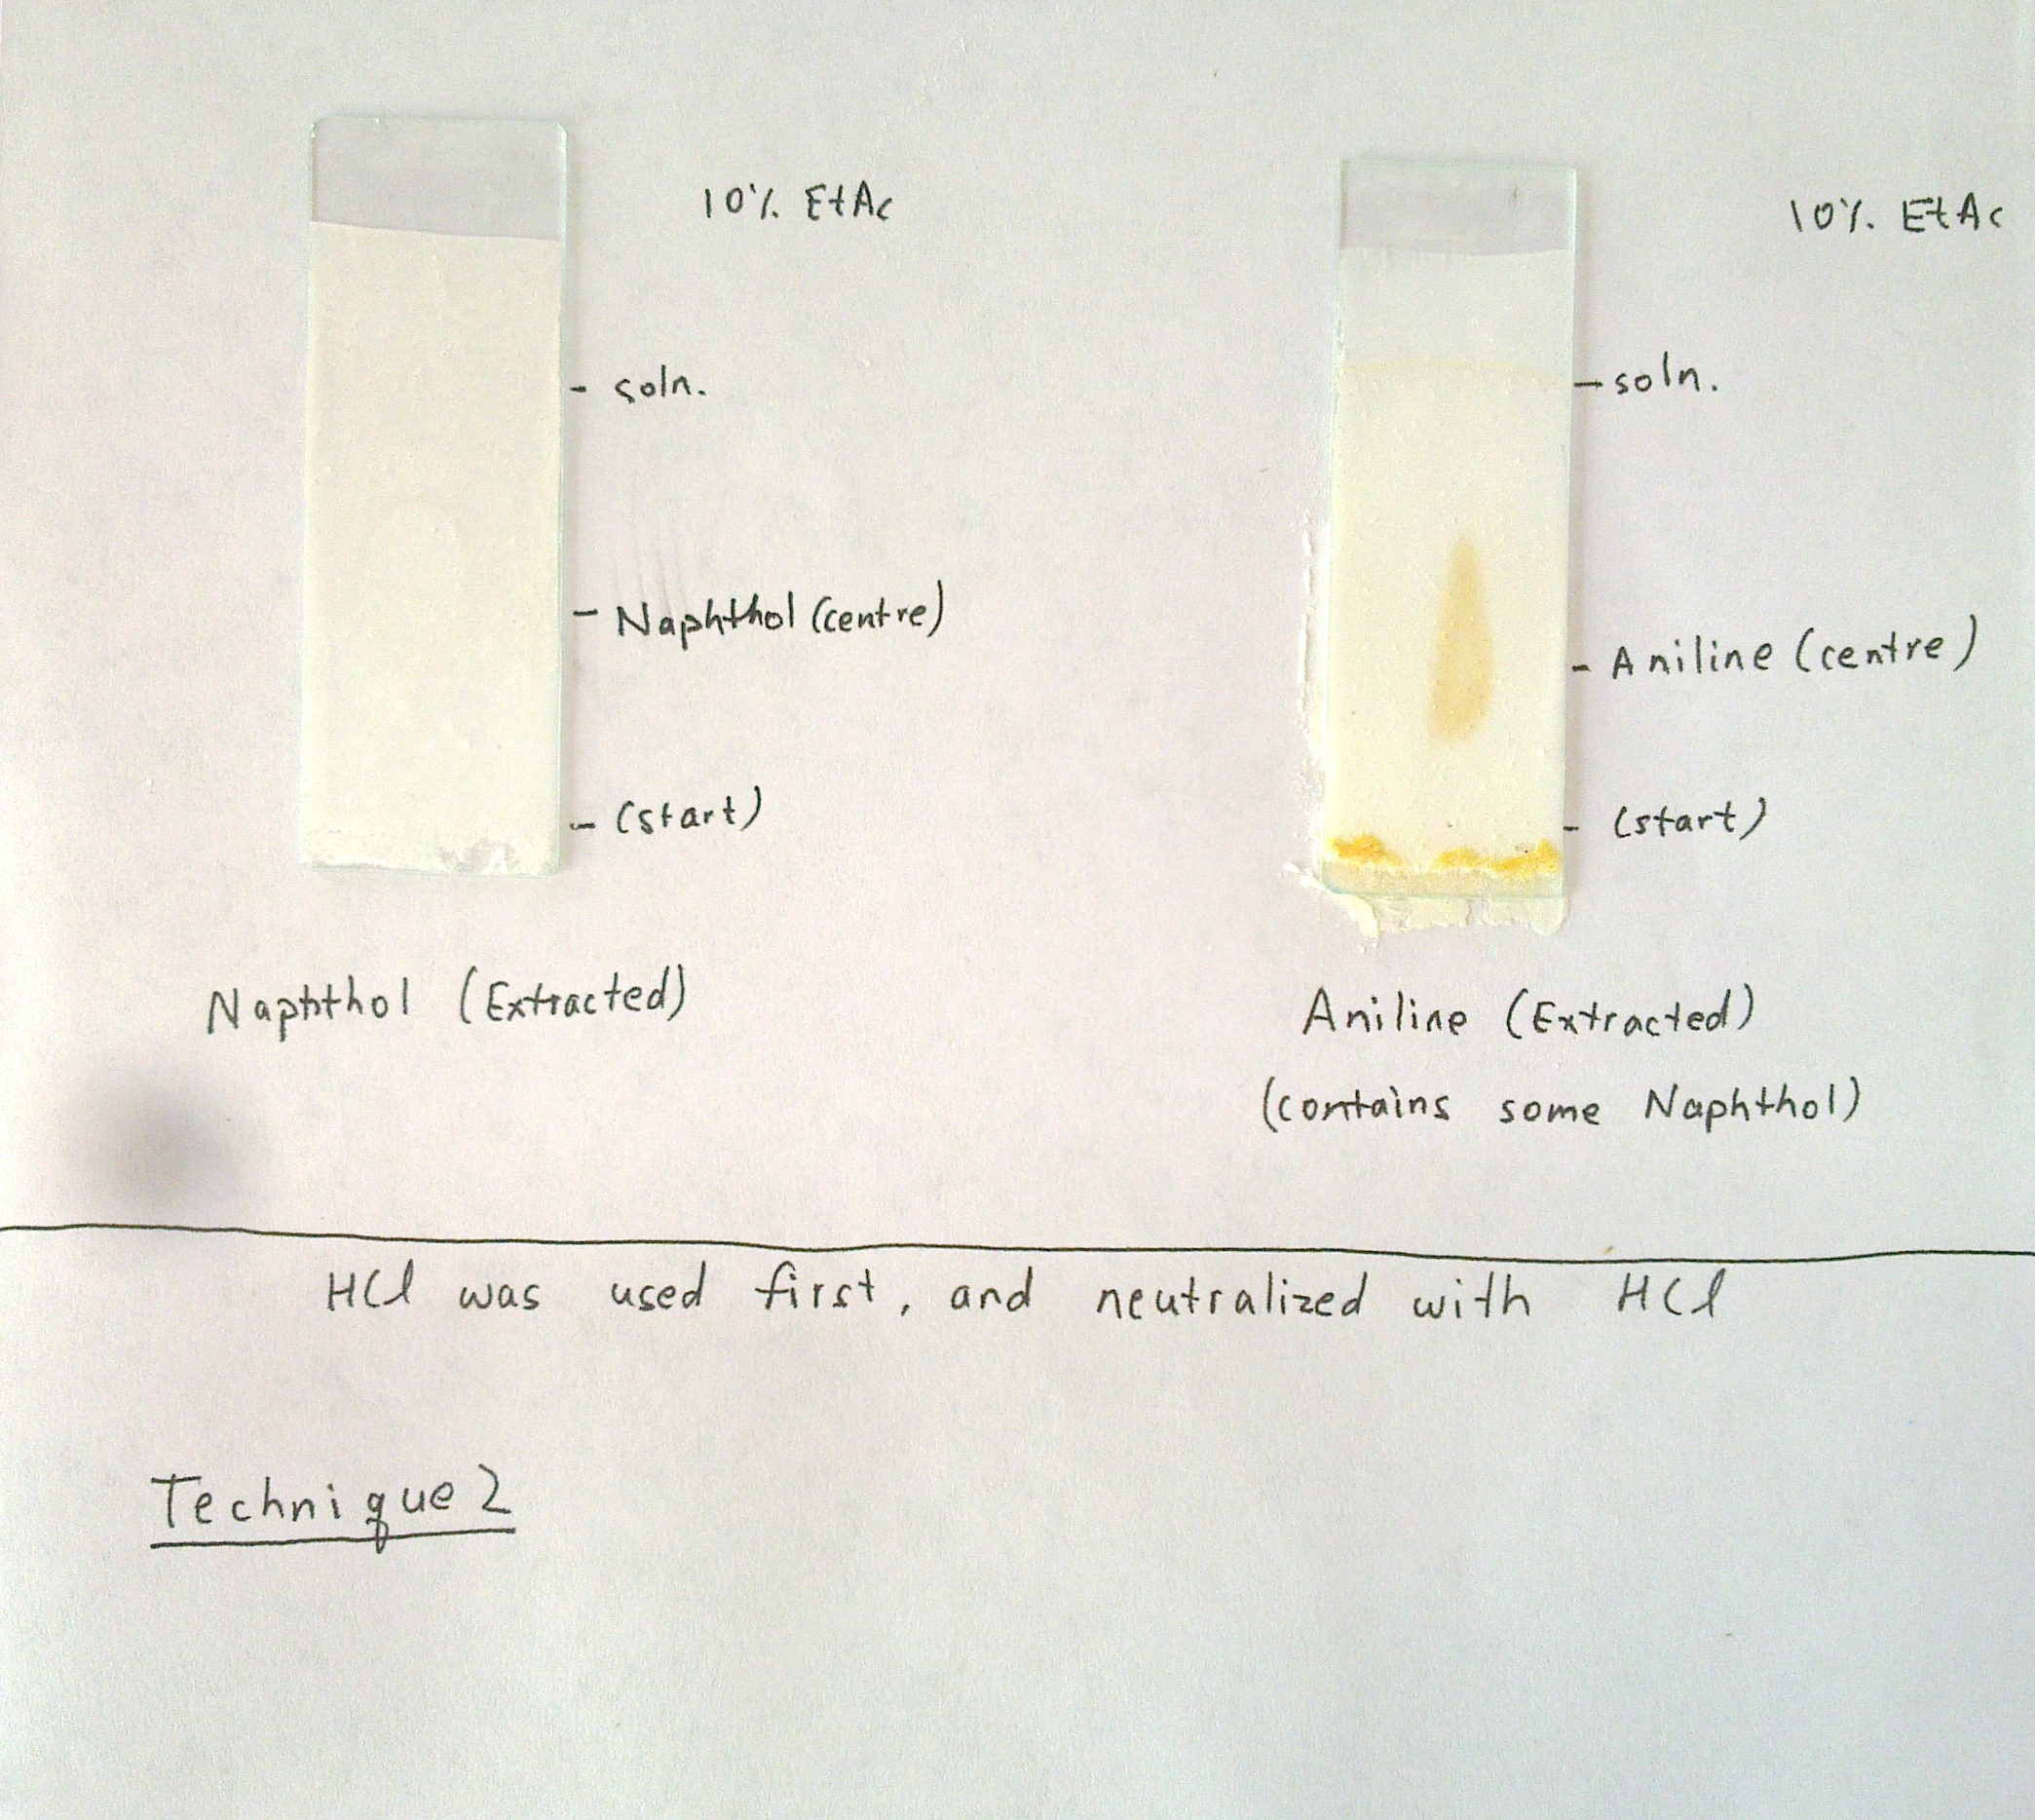
\includegraphics[width=1.0\linewidth]{gfx/e5_2}
	% 	\end{center}
	% \caption[TLCs Set 2]{\label{e5_2}}
	% \end{figure}